\documentclass[dvisvgm]{standalone}

\usepackage{tikz}
\usetikzlibrary {arrows.meta, positioning, automata}

\begin{document}

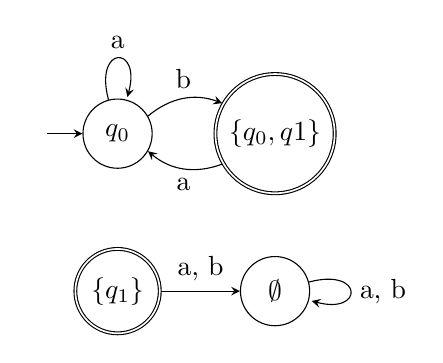
\begin{tikzpicture}[
    ->,
    >=stealth,
    node distance=2cm,
    initial text=$ $,
    on grid,
]

    \node[initial,   state]              (A) {$q_0$};
    \node[accepting, state, right =of A] (B) {$\{q_0, q1\}$};
    \node[accepting, state, below =of A] (C) {$\{q_1\}$};
    \node[           state, right =of C] (D) {$\emptyset$};

    \path
        (A) edge [loop above]       node {a}     (A)
        (A) edge [bend left, above] node {b}     (B)
        (B) edge [bend left, below] node {a}     (A)
        (C) edge [above]            node {a, b}  (D)
        (D) edge [loop right]      node {a, b}  (D)
    ;
\end{tikzpicture}

\end{document}